\appendix %% Start the appendices.
\chapter{Appendix}

\section{Comparison of Distance Measures and Prototype Selection Strategies on UCR datasets}
\label{sec:app-ucr}

As a part of this thesis, we tested multiple combinations of different distance measures and Feature DTW transformations, including various strategies for prototype selection on UCR datasets \cite{exp:UCRArchive2018}. In our implementation, we are using five-split cross-validation and comparing the average accuracy of each algorithm. For complete results, please see our repository \footnote{\url{https://github.com/H00N24/visual-analysis-of-big-time-series-datasets}}. Based on our results (Fig.~\ref{app:results-datasets}, Fig.~\ref{app:results-rank}), we make these conclusions:
\begin{itemize}
    \item The overall best distance measure is a combination of constrained DTW computed on the original time series and their derivations.
    \item Prototyped Feature DTW outperforms Prototyped Feature DTW.
    \item Random selection of prototypes can be a useful starting strategy.
\end{itemize}

\subsection*{Notation}
\subsubsection*{Distance measures:}
\begin{itemize}
    \item $dtw$ - Dynamic Time Warping \cite{met:dtw}
    \item $fdtw$ - Fast Dynamic Time Warping \cite{met:FastDTW}
    \item $sakoe\_chiba$ - DTW with Sakoe-Chiba constraint \cite{met:dtw-window}
    \item $itakura$ - DTW with Itakura constraint \cite{met:dtw-itakura}
    \item $dd\_distance\_measure\_\alpha$ - a combination of distance measure using the  original time series and their first derivatives ($ (1 - \alpha) * dist(x, y) + \alpha * dist(x', y') $) \cite{met:fDTW}
\end{itemize}
\subsubsection*{Prototype selection + Classification methods:}
\begin{itemize}
    \item $Random\_X$ - Randomly selecting $X\%$ of training data as prototypes ($Random\_10$, $Random\_30$, $Random\_50$) + Linear SVC
    \item $LassoSVC$ - Selecting prototypes with the highest importance from the Linear Support Vector Machine classifier with l1 penalization + Linear SVC
    \item $Tree$ - Selecting prototypes with the highest importance from the Extra Tree Classifier + Linear SVC
    \item $SVC$ - Using all prototypes + Linear SVC
    \item $1NN$ - Nearest Neighbor classifier using one closest neighbor
\end{itemize}
\begin{figure}[h]
    \centering
    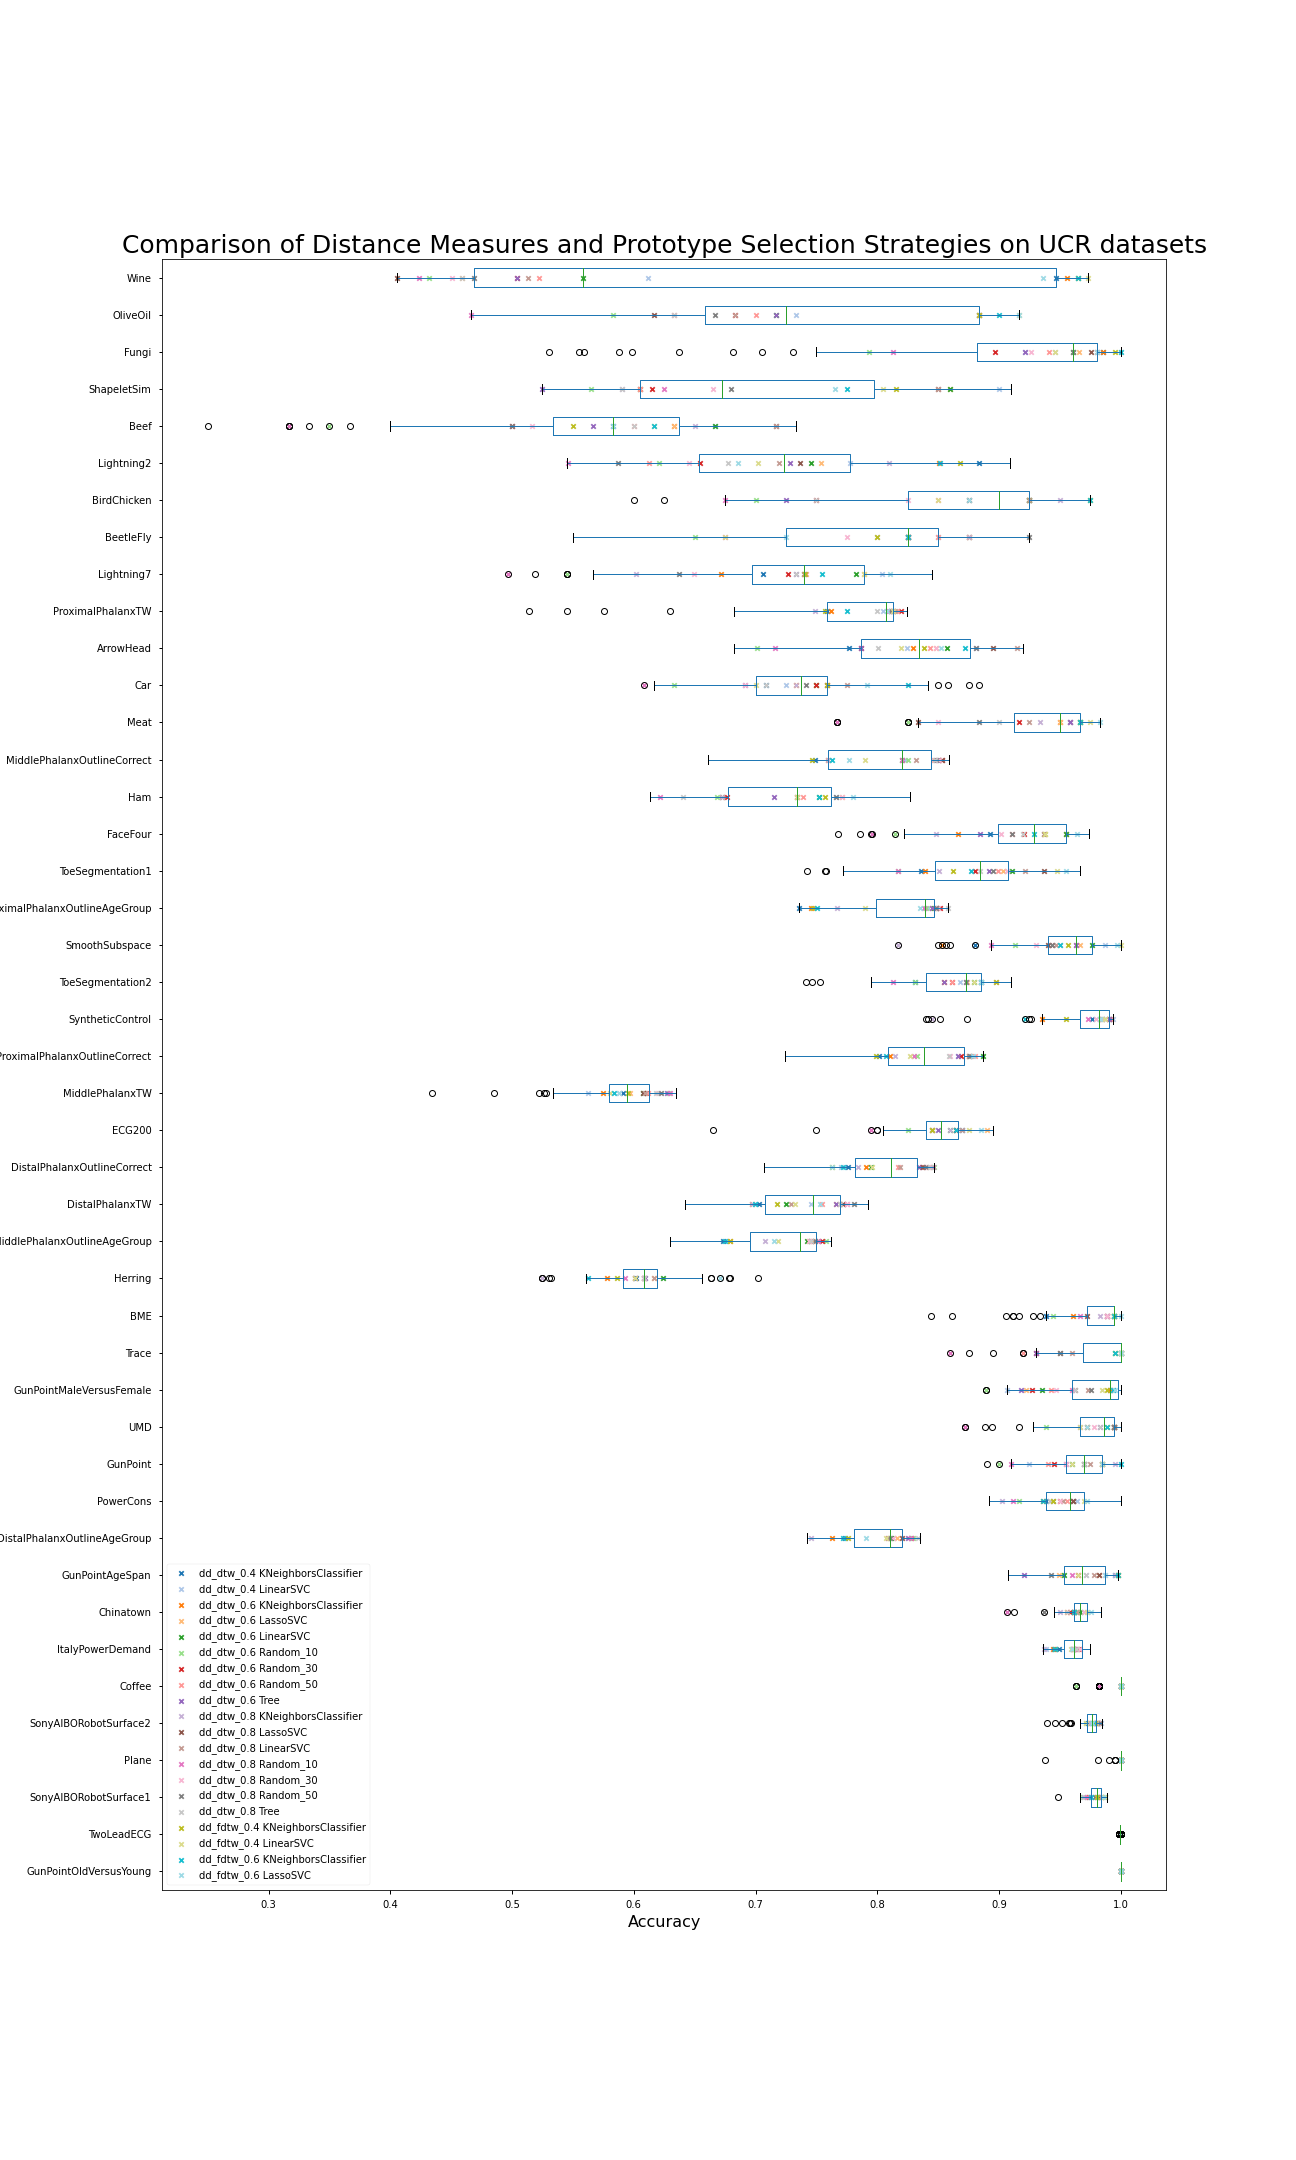
\includegraphics[width=\textwidth]{img/ucr_accuracy.png}
    \caption{Average accuracy of distance measures, prototype selection strategies, and classification algorithms on UCR datasets.}
    \label{app:results-datasets}
\end{figure}
\begin{figure}[h]
    \centering
    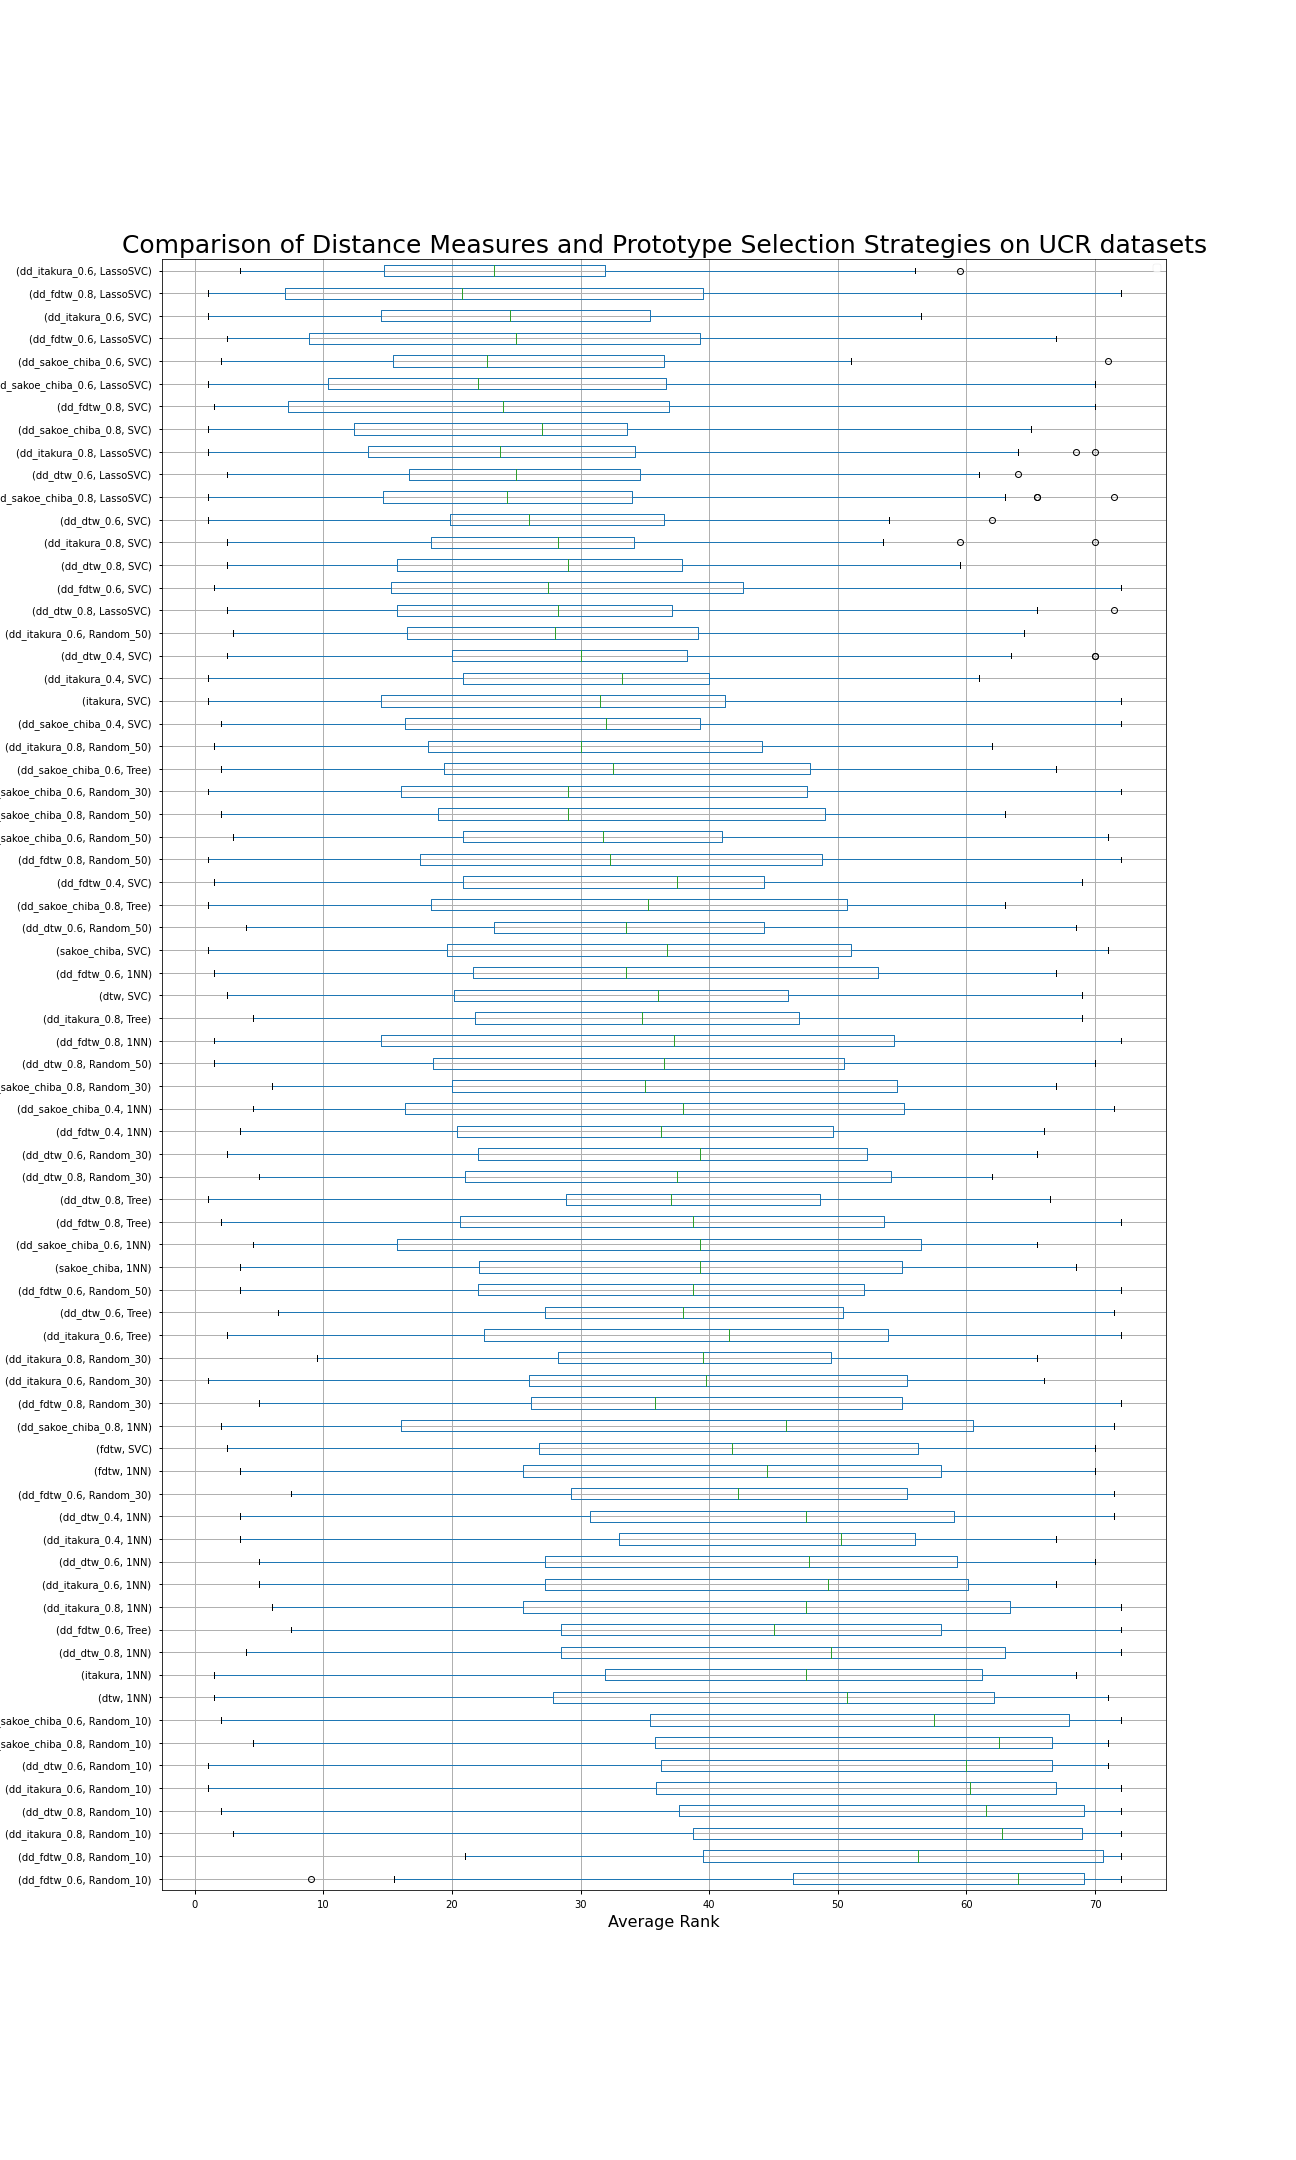
\includegraphics[width=\textwidth]{img/ucr_avg_rank.png}
    \caption{Average rank of combinations of distance measures and prototype selection strategies on UCR datasets.}
    \label{app:results-rank}
\end{figure}
